%%%%%%%%%%%%%%%%%%%%%%%%%%%%%%%%%%%%%%%%%
% baposter Landscape Poster
% LaTeX Template
% Version 1.0 (11/06/13)
%
% baposter Class Created by:
% Brian Amberg (baposter@brian-amberg.de)
%
% This template has been downloaded from:
% http://www.LaTeXTemplates.com
%
% License:
% CC BY-NC-SA 3.0 (http://creativecommons.org/licenses/by-nc-sa/3.0/)
%
%%%%%%%%%%%%%%%%%%%%%%%%%%%%%%%%%%%%%%%%%

%----------------------------------------------------------------------------------------
%	PACKAGES AND OTHER DOCUMENT CONFIGURATIONS
%----------------------------------------------------------------------------------------

\documentclass[landscape,a0paper,fontscale=0.285]{baposter} % Adjust the font scale/size here

\usepackage{graphicx} % Required for including images
\graphicspath{{figures/}} % Directory in which figures are stored
\usepackage{epstopdf}
\usepackage{amsmath} % For typesetting math
\usepackage{amssymb} % Adds new symbols to be used in math mode

\usepackage{verbatim}
\usepackage{booktabs} % Top and bottom rules for tables
\usepackage{enumitem} % Used to reduce itemize/enumerate spacing
\usepackage{palatino} % Use the Palatino font
\usepackage[font=small,labelfont=bf]{caption} % Required for specifying captions to tables and figures

\usepackage{multicol} % Required for multiple columns
\setlength{\columnsep}{1.5em} % Slightly increase the space between columns
\setlength{\columnseprule}{0mm} % No horizontal rule between columns

\usepackage{tikz} % Required for flow chart
\usetikzlibrary{shapes,arrows} % Tikz libraries required for the flow chart in the template

\newcommand{\compresslist}{ % Define a command to reduce spacing within itemize/enumerate environments, this is used right after \begin{itemize} or \begin{enumerate}
\setlength{\itemsep}{1pt}
\setlength{\parskip}{0pt}
\setlength{\parsep}{0pt}
}

\definecolor{lightblue}{rgb}{0.145,0.6666,1} % Defines the color used for content box headers

\begin{document}

\begin{poster}
{
headerborder=closed, % Adds a border around the header of content boxes
colspacing=1em, % Column spacing
bgColorOne=white, % Background color for the gradient on the left side of the poster
bgColorTwo=white, % Background color for the gradient on the right side of the poster
borderColor=lightblue, % Border color
headerColorOne=black, % Background color for the header in the content boxes (left side)
headerColorTwo=lightblue, % Background color for the header in the content boxes (right side)
headerFontColor=white, % Text color for the header text in the content boxes
boxColorOne=white, % Background color of the content boxes
textborder=roundedleft, % Format of the border around content boxes, can be: none, bars, coils, triangles, rectangle, rounded, roundedsmall, roundedright or faded
eyecatcher=true, % Set to false for ignoring the left logo in the title and move the title left
headerheight=0.1\textheight, % Height of the header
headershape=roundedright, % Specify the rounded corner in the content box headers, can be: rectangle, small-rounded, roundedright, roundedleft or rounded
headerfont=\Large\bf\textsc, % Large, bold and sans serif font in the headers of content boxes
%textfont={\setlength{\parindent}{1.5em}}, % Uncomment for paragraph indentation
linewidth=2pt % Width of the border lines around content boxes
}
%----------------------------------------------------------------------------------------
%	TITLE SECTION 
%----------------------------------------------------------------------------------------
%
{\includegraphics[height=4em]{logo_jlab.png}}
 % First university/lab logo on the left
{\bf\textsc{Searching for the Impetus of the EMC Effect.}\vspace{0.5em}} % Poster title
{\textsc{\{Jason Bane$^1$, Nadia Fomin,$^1$ Doug Higinbotham$^2$\} \hspace{12pt} \small{$^1$University of Tennessee $^2$Jefferson Lab}}} % Author names and institution
{\includegraphics[height=4em]{logo1.png}} % Second university/lab logo on the right




%----------------------------------------------------------------------------------------
%	OBJECTIVES
%----------------------------------------------------------------------------------------

\headerbox{Motivation}{name=motivation,column=0,row=0}{

In last few years, a large number of studies have tried to compare the EMC effect to Short Range Correlations (SRC). The current understanding of the EMC effect points to medium modification in quark distributions. While for SRCs, the correlated pairs of high momentum nucleons are the root cause.  

\vspace{1em}
 \textbf{Could the relationship between the EMC effect and SRC be high momentum nucleons? We will find out by investigating via a Monte Carlo simulation. }

\vspace{1.5em} % When there are two boxes, some whitespace may need to be added if the one on the right has more content
}

%----------------------------------------------------------------------------------------
%	INTRODUCTION
%----------------------------------------------------------------------------------------

\headerbox{Introduction}{name=introduction,column=1,span=2,row=0,bottomaligned=motivation}{
\begin{multicols}{2}
\begin{itemize}\compresslist

\item Lepton scattering experiments at CERN, SLAC, BCDMS, and Jlab
\item Use (e,$e\prime$) and (e,$e\prime$ p) experiments to study the EMC effect and SRCs.
\item EMC effect discovered in the early 80s by European Muon Collaboration\cite{Norton}. 
\item EMC effect: Slope in A/D ratios between 0.3 and 0.7 x$_B$.
\item SRCs - from correlated high pairs of momentum nucleons.
\item SRCs: x$_B$ greater than 1.4 plateaus.


\end{itemize}
\begin{center}
\includegraphics[width=0.9\linewidth]{EMC_1}
\vspace{-1em}
\captionof{figure}{A/D ratio of cross sections. \cite{cern}}
\end{center}


\end{multicols}
}

%----------------------------------------------------------------------------------------
%	RESULTS 1
%----------------------------------------------------------------------------------------

\headerbox{Simulation}{name=sim,column=3,row=0,bottomaligned=motivation}{
%The Monte Carlo Simulation scatters an electron off of a moving proton by completing the following steps:

\begin{itemize}\compresslist

\item Randomly select the proton's direction relative to the electron beam.
\item Select the momentum of the proton using a given momentum distribution.
\item Complete a set of transformations to move to the rest frame of the target proton.
\item Elastically scatter the electron to a randomly selected angle, followed by the scattered electron radiating some of its energy away to move into the inelastic scattering regime. 
\item Transform back to the lab frame for final analysis.
\end{itemize}
}


%----------------------------------------------------------------------------------------
%   Transformation
%----------------------------------------------------------------------------------------

\headerbox{Transformation}{name=trans,column=0,below=motivation}{ % This block's bottom aligns with the bottom of the conclusion block


\begin{multicols}{2}
\vspace{-2em}
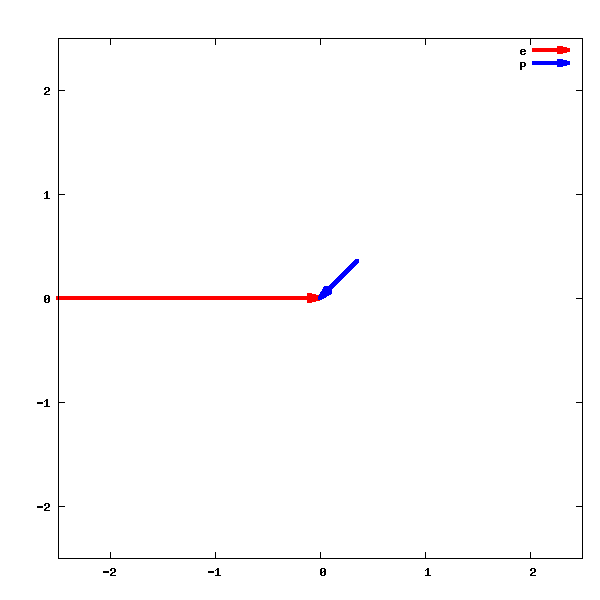
\includegraphics[width=0.95\linewidth]{Initial}
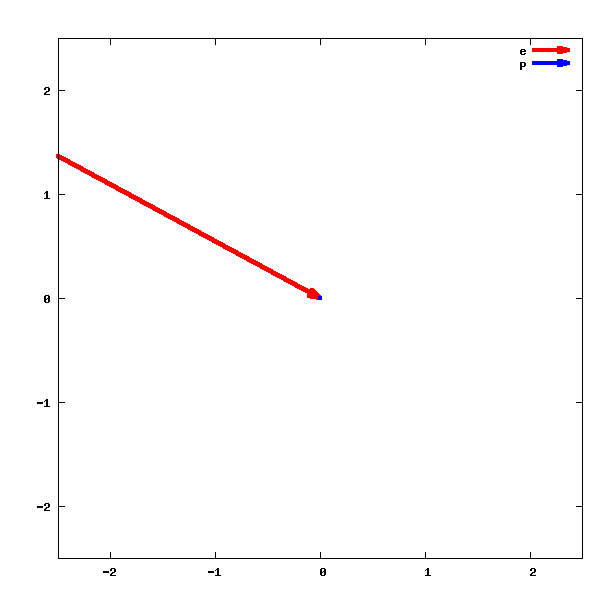
\includegraphics[width=0.95\linewidth]{boosted}
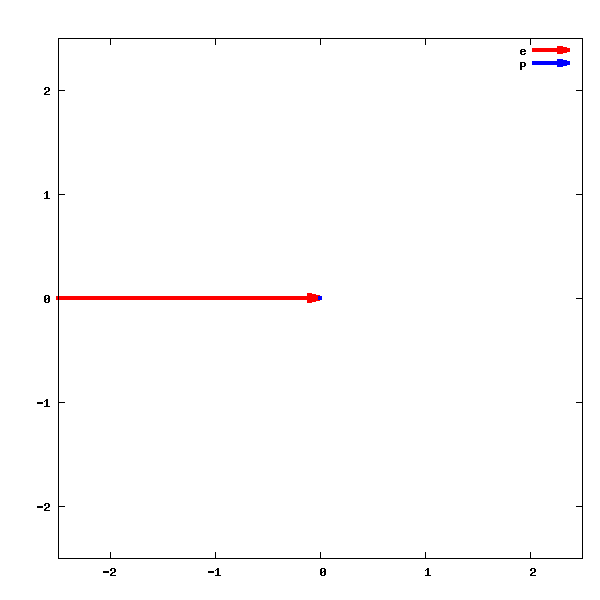
\includegraphics[width=0.95\linewidth]{beforescattering}

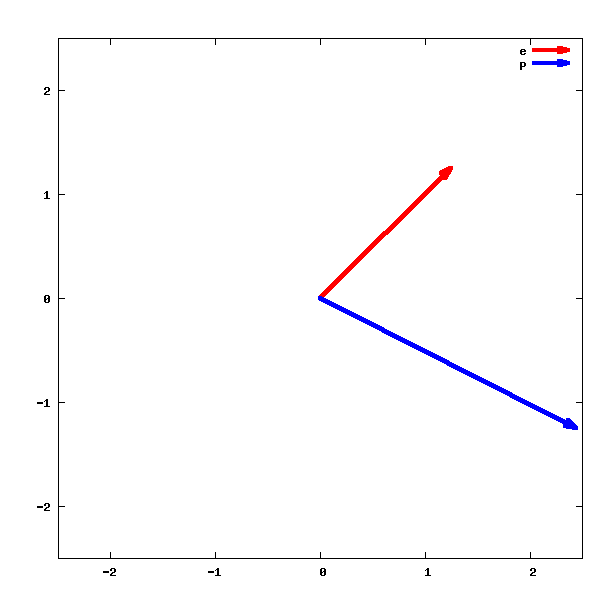
\includegraphics[width=0.95\linewidth]{afterscatter}
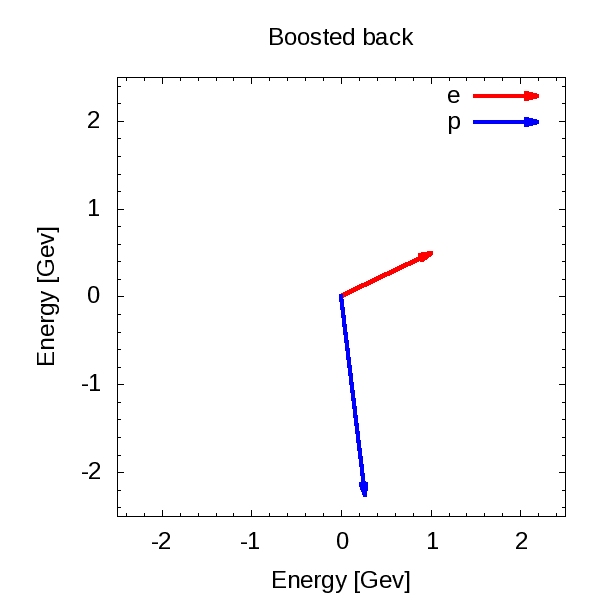
\includegraphics[width=0.95\linewidth]{boostedback}
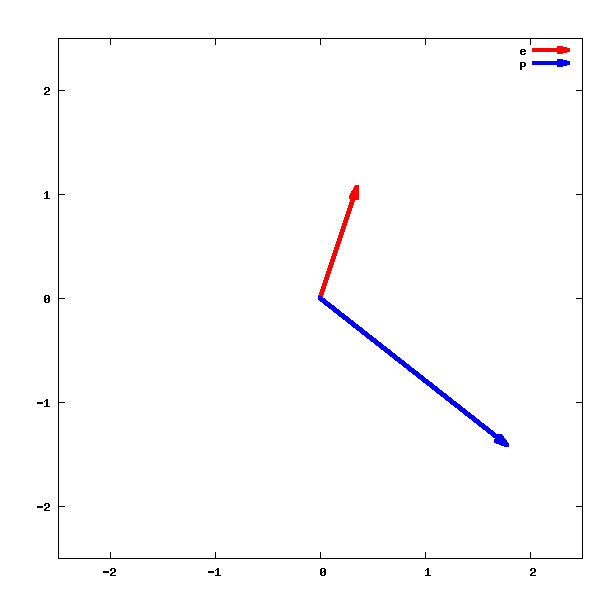
\includegraphics[width=0.95\linewidth]{final}
\end{multicols} 


}


%----------------------------------------------------------------------------------------
%	RESULTS 2
%----------------------------------------------------------------------------------------

\headerbox{Proton Momentum }{name=pmom,column=1,span=1,below=motivation,bottomaligned=trans}{ 
\includegraphics[width=1\linewidth]{Av18_2_4_9_12.eps}


%\hspace{5em}
%\includegraphics[width=.5\linewidth]{Mo_dist_run_0.eps}

%\vspace{-.250em}

%\includegraphics[width=.47\linewidth]{Mo_dist_run_1.eps}

%\vspace{-7.05em}
%\hspace{11em}
%\includegraphics[width=.47\linewidth]{Mo_dist_run_10.eps}


\vspace{-1.1em}
\begin{itemize}[leftmargin=*]\compresslist

\item These distributions are made from the Av18 calculations for Single Nucleon Momentum Distributions\cite{av18,av18_2}.
\item C12 - A run that uses the Av18 results for Carbon 12 with .    
\item He4 has a slight increase in the probability of the  higher momentum nucleon.
\item Run 2 has a dramatic increase in probability of the  higher momentum nucleon. 
\item Next step: Match the momentum distributions used in the simulation to actual momentum distributions found in nuclei.   
 
\end{itemize}
}


%----------------------------------------------------------------------------------------
%	CONCLUSION
%----------------------------------------------------------------------------------------

\headerbox{Results}{name=conclusion,column=2,span=2,below=sim,bottomaligned=trans}{
\vspace{.4cm}
\begin{multicols}{3}

\addtolength{\linewidth}{3in}

\includegraphics[width=0.4 \linewidth]{XbWL_1_0.eps}
\includegraphics[width=0.4 \linewidth]{XbWL_10_0.eps}

\hspace{-2em}\includegraphics[width=0.5 \linewidth]{RatioW_lab_1_0.eps}

\hspace{-2em}\includegraphics[width=0.5\linewidth]{RatioW_lab_10_0.eps}


\columnbreak

\begin{itemize}[leftmargin=*]

\item Top Left: Weighted counts for\\ the Base Run and Run 1. 

\item Top Right: Ratio of the results\\ for runs 1 and the Base Run. 

\item Bottom Left: Weighted counts\\ for the Base Run and Run 2. 

\item Bottom Right: Ratio of the\\ results for runs 2 and the Base. 
\vspace{-1em}
\item Comparing the results for \\
the two ratios. Notice the lack\\ 
of change in the ratio for run\\
1 and the Base run and the\\ 
strong downward slope from \\
0.3 to 0.7 in x$_B$ for run 2 and \\
the base run. 



\end{itemize}
\end{multicols}
}



%----------------------------------------------------------------------------------------
%	REFERENCES
%----------------------------------------------------------------------------------------

\headerbox{References}{name=references,span=2,column=0,above=bottom,bottomaligned=conc}{
\begin{multicols}{2}
\renewcommand{\section}[2]{\vskip 0.05em} % Get rid of the default "References" section title
\nocite{*} % Insert publications even if they are not cited in the poster
\small{ % Reduce the font size in this block
\bibliographystyle{unsrt}
\bibliography{sample}


}\end{multicols}
}

%----------------------------------------------------------------------------------------
%	FUTURE RESEARCH
%----------------------------------------------------------------------------------------

\headerbox{Conclusion}{name=conc,column=2,span=2,above=bottom}{ 

\begin{multicols}{2}
Results produced from the simulation show there is a correlation between the weighted counts in x$_B$ for this inelastic scattering process and the momentum distribution used to simulate the momentum of the target nucleon. 


\end{multicols}
}








\end{poster}

\end{document}